\documentclass[conference]{IEEEtran}

\usepackage[T5]{fontenc}
\usepackage[utf8]{inputenc}
\usepackage{graphicx}
\usepackage{amsmath, amssymb}
\usepackage{booktabs}
\usepackage{siunitx}
\usepackage{cite}
\usepackage{placeins}
\usepackage{subcaption}
\usepackage{float}
\usepackage{tikz}
\usepackage{xcolor}
\usetikzlibrary{shapes.geometric, arrows.meta, positioning, fit, backgrounds}

\title{Design and Implementation of an Interactive Wrist Rehabilitation System Integrated with a Web-based Game}

\author{
\IEEEauthorblockN{ Tran Quoc Loc, Tran Quang Minh, Bui Quang Huy, Le Quoc Viet, Nguyen Phan Kien$^{*}$ }
\IEEEauthorblockA{\textit{Students of Biomedical Engineering}, School of Electrical and Electronic Engineering (SEEE), HUST\\
Hanoi, Vietnam\\
Email: \{loc.tq233966, minh.tq233971, huy.bq.... viet.lq233987\}@sis.hust.edu.vn}
*Corresponding author: 
}

\begin{document}
\maketitle

\begin{abstract}
Wrist rehabilitation after stroke is crucial for restoring patients' daily living activities; however, barriers such as high costs and the complexity of local software middleware currently limit home-based exercises. This paper proposes a low-cost 1-DOF robotic rehabilitation system based on a "Zero-Setup" architecture, allowing therapy sessions to be deployed directly via web browsers without complex software installation. The system utilizes a Master-Slave structure combined with a PID controller and an S-Curve PWM algorithm to eliminate static friction, ensuring smooth motion trajectories for passive range-of-motion exercises. The core contribution is the exploitation of the Web Serial API to establish a direct bridge between the Arduino hardware and an HTML5 Canvas-based game, providing immersive visual biofeedback. Experimental results confirm that the system's communication latency remains consistently under 50ms, ensuring real-time interactivity. Furthermore, hardware-level Range of Motion (ROM) safety bounding mechanisms are implemented to eliminate the risk of secondary injuries. This solution demonstrates the high feasibility of a low-cost, safe, and accessible telerehabilitation model for patients at home.
\end{abstract}

\section{Introduction}

Stroke and related neurological disorders are among the leading causes of long-term motor impairment, severely limiting patients' ability to perform Activities of Daily Living (ADL). Given the critical role of the wrist in fine motor skills, dexterity, and grasping, wrist rehabilitation is a fundamental focus in post-stroke physical therapy. Traditional rehabilitation methods rely heavily on one-on-one sessions with therapists, which are labor-intensive, expensive, and geographically challenging for patients requiring long-term daily care \cite{vo2024design, omarkulov2016preliminary}.

To address these limitations, Robot-Assisted Therapy (RAT) combined with gamification has emerged as a promising solution \cite{tolks2024role}. By translating physical rehabilitation movements into inputs for virtual games, these systems provide real-time biofeedback, create data-driven monitoring mechanisms, and significantly enhance patient motivation and therapy adherence. Although the clinical efficacy of such systems is well-documented through large-scale meta-analyses \cite{park2025effects}, transitioning these mechatronic devices from clinical environments to home-based "Telerehabilitation" remains a major challenge.

A significant barrier to widespread home adoption is the technological complexity associated with device setup. Most current rehabilitation robots require complex local software ecosystems, middleware (such as Python scripts, MATLAB environments, or custom Serial drivers), and difficult calibration procedures. This creates a steep learning curve for non-technical patients. Furthermore, designing a low-cost mechatronic system capable of providing smooth kinematic assistance while accurately measuring dynamic interactions—such as patient-applied torque and force—presents a substantial technical hurdle.

In this study, we present the design and implementation of a low-cost, gamified, "Zero-Setup" wrist rehabilitation device. Completely bypassing the need for middleware applications, the architecture leverages the Web Serial API to establish a direct, low-latency bridge between the microcontroller-driven mechatronic system and an HTML5 browser-based game environment. The core contributions of this paper are three-fold:
\begin{itemize}
    \item \textbf{Zero-Setup Architecture:} Leveraging Web Serial communication to enable immediate therapy without driver installation, accessible via any modern web browser.
    \item \textbf{Master-Slave Kinematics and Hardware Safety:} An integrated PID position tracking algorithm providing asymmetric assistance, reinforced by strict hardware-level Range of Motion (ROM) safety limits enforced natively on the microcontroller.
    \item \textbf{Integrated Torque Monitoring:} Implementation of a high-resolution current-sensing feedback loop utilizing an INA219 sensor and a three-stage cascaded digital filter. This enables real-time torque estimation, facilitating the transition from passive assistance to active-resistive therapy protocols.
\end{itemize}

The remainder of this paper is organized as follows: Section II provides an overview of Related Work. Section III proposes the Methodology, including hardware design, control algorithms, and web software integration. Section IV evaluates the Experiments and Results, and Section V summarizes the key conclusions.

\section{Related Work}

The application of robotics in upper limb and wrist rehabilitation has attracted significant attention in recent decades. Numerous robotic rehabilitation systems have been developed with various degrees of freedom (DOF), typically utilizing cable-driven mechanisms or parallel structures. Although these systems provide sophisticated force assistance (e.g., Impedance Control), they are often bulky, expensive, and limited to clinical settings or specialized therapy centers \cite{park2025effects}. This clinical confinement inadvertently restricts the frequency of exercise for patients who require continuous daily recovery.

To transition toward a home-based Telerehabilitation model, several recent studies have proposed compact robotic prototypes integrated with virtual game environments \cite{tolks2024role}. These approaches often focus on 1-DOF designs using current sensing for torque estimation or applying Proportional-Integral-Derivative (PID) algorithms to assist motion trajectories via PC-based game development tools such as Python, Unity, or MATLAB \cite{vo2024design, nikafrooz2017design}.

However, a common limitation of these systems is their reliance on locally installed middleware. Patients or caregivers are often required to install Serial COM drivers, download executable files, or even configure programming language environments. This technical barrier reduces user-friendliness and limits the independent deployment of these systems at home for elderly patients.

In contrast to previous studies, our system introduces a non-traditional approach to Telerehabilitation: completely eliminating middleware through the \textbf{Web Serial API}. The "Zero-Setup" concept allows the microcontroller to communicate directly with an HTML5-based open-source game environment, creating a seamless experience: the patient simply connects the device via USB and opens a browser tab. Furthermore, we propose a Master-Slave kinematic architecture combined with mechanical safety boundaries implemented directly on the microcontroller, making home training not only convenient but also inherently safe.

\section{Proposed Methodology}

The proposed wrist rehabilitation system comprises three main subsystems: (A) Mechatronic design, (B) Kinematic control strategy, and (C) Zero-Setup software architecture. This combination aims to create a low-cost assistive device that simulates the safety and flexibility of industrial robotic systems.



% ===== SYSTEM BLOCK DIAGRAM =====
\begin{figure}[!t]
\centering
\resizebox{\columnwidth}{!}{%
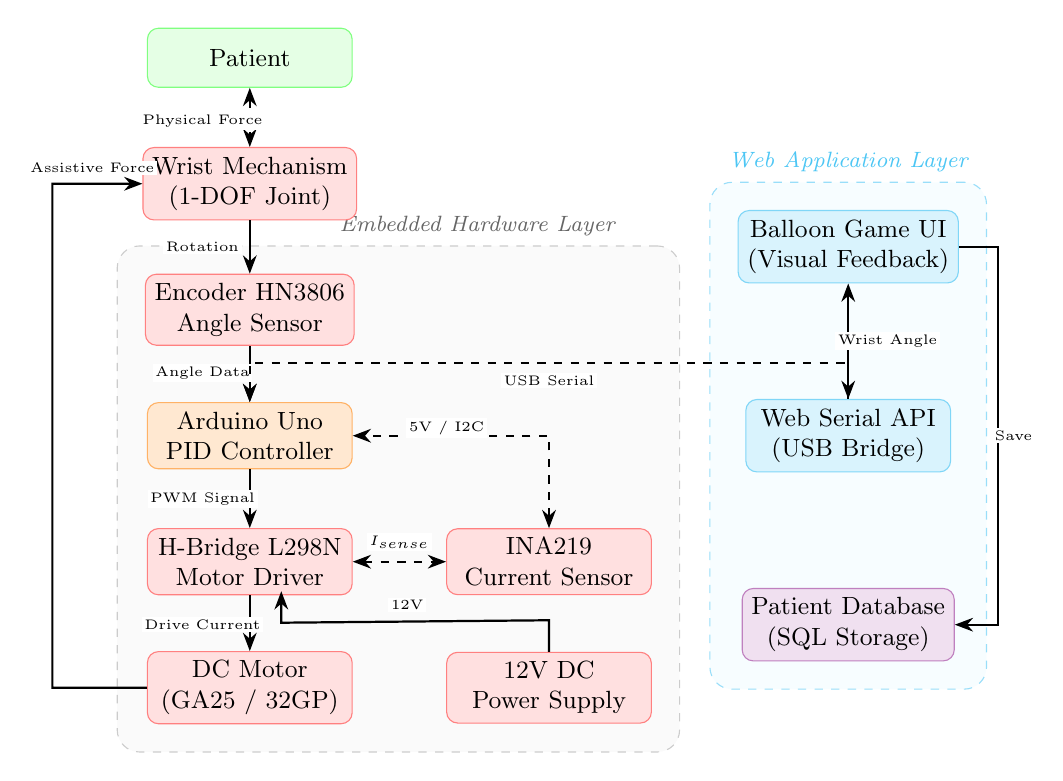
\begin{tikzpicture}[
    box/.style  = {rectangle, rounded corners=4pt, draw,
                   minimum width=2.6cm, minimum height=0.75cm,
                   align=center, font=\small},
    hwbox/.style  = {box, fill=red!12,    draw=red!50},
    mcubox/.style = {box, fill=orange!18, draw=orange!60},
    swbox/.style  = {box, fill=cyan!15,   draw=cyan!50},
    dbbox/.style  = {box, fill=violet!12, draw=violet!50},
    pbox/.style   = {box, fill=green!10,  draw=green!50},
    arr/.style    = {-Stealth, thick},
    darr/.style   = {Stealth-Stealth, thick, dashed}
]

%% ---- COLUMN A: Main hardware pipeline ----
\node[pbox]   (patient) at (0,    0)   {Patient};
\node[hwbox]  (mech)    at (0,   -1.6) {Wrist Mechanism\\(1-DOF Joint)};
\node[hwbox]  (encoder) at (0,   -3.2) {Encoder HN3806\\Angle Sensor};
\node[mcubox] (arduino) at (0,   -4.8) {Arduino Uno\\PID Controller};
\node[hwbox]  (l298n)   at (0,   -6.4) {H-Bridge L298N\\Motor Driver};
\node[hwbox]  (motor)   at (0,   -8.0) {DC Motor\\(GA25 / 32GP)};

%% ---- COLUMN B: Sensors at same y-levels ----
\node[hwbox]  (ina219)  at (3.8, -6.4) {INA219\\Current Sensor};
\node[hwbox]  (power)   at (3.8, -8.0) {12V DC\\Power Supply};

%% ---- COLUMN C: Web Application ----
\node[swbox]  (game)    at (7.6, -2.4) {Balloon Game UI\\(Visual Feedback)};
\node[swbox]  (serial)  at (7.6, -4.8) {Web Serial API\\(USB Bridge)};
\node[dbbox]  (db)      at (7.6, -7.2) {Patient Database\\(SQL Storage)};

%% =============================================
%% ARROWS - Column A (vertical pipeline)
%% =============================================
\draw[darr] (patient) -- (mech);
\node[font=\tiny,fill=white,inner sep=1pt] at (-0.6,-0.8) {Physical Force};

\draw[arr] (mech)    -- (encoder);
\node[font=\tiny,fill=white,inner sep=1pt] at (-0.6,-2.4) {Rotation};

\draw[arr] (encoder) -- (arduino);
\node[font=\tiny,fill=white,inner sep=1pt] at (-0.6,-4.0) {Angle Data};

\draw[arr] (arduino) -- (l298n);
\node[font=\tiny,fill=white,inner sep=1pt] at (-0.6,-5.6) {PWM Signal};

\draw[arr] (l298n)   -- (motor);
\node[font=\tiny,fill=white,inner sep=1pt] at (-0.6,-7.2) {Drive Current};

%% Feedback: Motor -> Wrist (3-segment, EXACT rectangular)
%% motor y=-8.0, mech y=-1.6, diff=6.4 exactly
\draw[arr] (motor.west)
    -- ++(-1.2,0)
    -- ++(0,6.4)
    -- (mech.west);
%% Label above the TOP horizontal segment
\node[font=\tiny,fill=white,inner sep=1pt] at (-2.0,-1.4) {Assistive Force};

%% =============================================
%% ARROWS - Column B
%% =============================================

%% 1. L298N ↔ INA219: bidirectional (current sensing shunt in series)
\draw[darr] (l298n.east) -- (ina219.west);
\node[font=\tiny,fill=white,inner sep=1pt] at (1.9,-6.15) {$I_{sense}$};

%% 2. 12V Power → L298N: enter from BOTTOM of l298n (below 'r' in Driver ≈ x=0.4)
%%    power.north(3.8,-7.625) → up 0.45 → horiz to x=0.4 → up into l298n south
\draw[arr] (power.north) -- ++(0,0.4) -- (0.4,-7.175) -- (0.4,-6.775);
\node[font=\tiny,fill=white,inner sep=1pt] at (2.0,-6.95) {12V};

%% 3. Arduino ↔ INA219: 5V power + I2C data
\draw[darr, sharp corners] (ina219.north) |- (arduino.east);
\node[font=\tiny,fill=white,inner sep=1pt] at (2.5,-4.7) {5V / I2C};

%% =============================================
%% ARROWS - Column C (Web layer)
%% =============================================
%% Arduino <-> Web Serial (horizontal, clear path above INA219)
\draw[darr] (arduino.north) -- ++(0,0.5) -| (serial.north);
\node[font=\tiny,fill=white,inner sep=1pt] at (3.8,-4.1) {USB Serial};

%% Web Serial → Game (vertical up)
\draw[arr] (serial.north) -- (game.south);
\node[font=\tiny,fill=white,inner sep=1pt] at (8.1,-3.6) {Wrist Angle};

%% Game → Database (route right side)
\draw[arr] (game.east)  -- ++(0.5,0)
           |- (db.east);
\node[font=\tiny,fill=white,inner sep=1pt] at (9.7,-4.8) {Save};

%% =============================================
%% BACKGROUND LAYER BOXES
%% =============================================
\begin{scope}[on background layer]
    \node[draw=gray!40, dashed, rounded corners=8pt, fill=gray!4,
          inner sep=10pt,
          fit=(encoder)(arduino)(l298n)(motor)(ina219)(power),
          label={[font=\footnotesize\itshape,text=black!60,xshift=1.0cm]above:Embedded Hardware Layer}] {};
    \node[draw=cyan!40, dashed, rounded corners=8pt, fill=cyan!3,
          inner sep=10pt,
          fit=(serial)(game)(db),
          label={[font=\footnotesize\itshape,text=cyan!70]above:Web Application Layer}] {};
\end{scope}

\end{tikzpicture}
}%
\caption{System Architecture Block Diagram of the Wrist Rehabilitation Device.}
\label{fig:blockdiagram}
\end{figure}
% ================================

\subsection{Mechanical Design and Hardware}

In robotic wrist rehabilitation systems, determining the number of Degrees of Freedom (DOF) is a decisive factor in balancing therapeutic efficacy and control system complexity. While previous studies have developed 3-DOF structures to comprehensively simulate wrist movements, this research proposes an optimized solution focusing specifically on the Flexion/Extension (FE) axis.

\begin{figure}[!t]
\centering
\includegraphics[width=0.8\columnwidth]{cung1.png}
\caption{Biomechanics of the wrist Flexion/Extension (FE) axis movement.}
\label{fig:biomechanics}
\end{figure}

Flexion/Extension (FE) is the most critical and highest-amplitude movement axis of the wrist, playing a key role in hand positioning for functional tasks. During flexion, the hand moves toward the palmar side with a normal physiological range of up to approximately $70^\circ - 80^\circ$. Conversely, extension occurs when the back of the hand moves toward the forearm, reaching a similar limit of about $70^\circ - 85^\circ$. The coordinated interaction between the proximal and distal carpal bones allows for a dynamic pivot axis, reducing concentrated pressure on a single bony point. To naturally simulate the FE axis, the device must accommodate a standard Range of Motion (ROM) of $70^\circ$ flexion and $70^\circ$ extension to ensure the ability to perform Activities of Daily Living (ADLs).

\begin{figure}[!t]
\centering
\includegraphics[width=0.8\columnwidth]{cung2.png}
\caption{Mechanical structure of the sector gear and central support frame.}
\label{fig:sector_gear}
\end{figure}

The core of the hardware design lies in converting the rotation of the drive system into the biological curved trajectory of the wrist. The device utilizes a large-radius sector gear mechanism coordinated with a central support frame. The arc structure itself serves as a mechanical stop, preventing excessive wrist flexion or extension and ensuring maximum patient safety in case of software failure.

\begin{figure}[!t]
\centering
\includegraphics[width=0.8\columnwidth]{cung3.png}
\caption{Alignment of the pivot center with the radiocarpal joint.}
\label{fig:alignment}
\end{figure}

A fundamental design point is aligning the pivot center of the sector gear with the instantaneous center of rotation of the radiocarpal (wrist) joint. The support structure is calculated to create a clearance space beneath the rotation axis, allowing the patient's forearm and wrist to be positioned centrally. In the mechanical architecture of the 1-DOF wrist rehabilitation robot, the transmission system between the GA25 motor and the gear acts as the core actuation system, determining the effectiveness of the exercise routines. Additionally, an encoder is attached to the shaft of the pinion gear opposite the motor. As the sector gear rotates, it drives the encoder. Based on the known transmission ratio, the system can accurately calculate the handle's rotation angle with extremely high resolution (the encoder resolution multiplied by the gear ratio).

\subsection{Control System Design and Assistive Force Monitoring}

The prototype system is built upon a closed-loop feedback control structure, utilizing an Arduino Nano microcontroller as the central processing unit to optimize size and real-time responsiveness. The primary actuator is a GA25 DC geared motor, controlled via pulse-width modulation (PWM) signals to provide the necessary torque for wrist exercise routines.

To ensure precision in joint angle positioning, a high-resolution HN3806 optical rotary encoder (600 pulses/revolution) is mounted coaxially with the device's output shaft. Utilizing the HN3806 encoder allows the system to monitor position error with a resolution of up to $0.15^\circ$, providing critical input data for the assistive motion algorithm.

To guarantee smooth and accurate trajectory following for the rehabilitation mechanism, the system implements a Position PID controller in a real-time environment. In closed-loop feedback control systems, the PID controller plays a leading role due to its flexible adjustability. The general mathematical equation for a PID controller in the continuous time domain is expressed as follows:

\begin{equation}
u(t) = K_p e(t) + K_i \int_0^t e(\tau)d\tau + K_d \frac{de(t)}{dt}
\label{eq:pid_continuous}
\end{equation}

Where:
\begin{itemize}
    \item $e(t)$: Instantaneous error between the Setpoint and the Process Variable.
    \item $K_p$ (Proportional gain): Produces a control signal proportional to the current error, providing immediate feedback.
    \item $K_i$ (Integral gain): Eliminates steady-state error by accumulating error over time.
    \item $K_d$ (Derivative gain): Predicts error variation trends to adjust response speed and minimize overshoot.
\end{itemize}

In the Arduino Nano microcontroller, the PID algorithm is implemented in a discrete form to match the system's sampling period. Therefore, the continuous equation needs to be converted into a practical difference form. The output signal $output(k)$ at the $k^{th}$ sampling cycle is calculated as:

\begin{equation}
output(k) = K_p \cdot e(k) + K_i \sum_{i=0}^k e(i) + K_d [e(k) - e(k-1)]
\label{eq:pid_discrete}
\end{equation}

In the wrist rehabilitation device, to ensure safety and motion stability, we selected specific parameters as follows:
\begin{itemize}
    \item \textbf{Proportional gain $K_p = 1.0$}: Set at a low level to generate a gentle initial response, preventing sharp force impulses that could cause secondary injuries to the patient.
    \item \textbf{Integral gain $K_i = 0.15$}: Functions to compensate for the static friction and gravity components of the mechanical mechanism, ensuring the system reaches a steady state without excessive oscillations around the target position.
    \item \textbf{Derivative gain $K_d = 2.0$}: Configured with the highest value among the parameters to act as a "kinematic brake" (damping). Prioritizing the derivative component enhances the system's vibration resistance, ensuring a smooth wrist motion trajectory and a soft stop at the designated position.
\end{itemize}

However, small DC motors like the GA25 often exhibit significant static friction ($F_S$), leading to a notable "dead-zone" where the motor only produces a whining sound or slight vibration without rotating when the input voltage is below a critical threshold. To fundamentally address this issue, a non-linear PWM mapping algorithm (S-Curve PWM) is proposed to overcome the physical limitations of the motor and ensure maximum smoothness for the patient \cite{pezent2017design}. This strategy includes dead-zone compensation combined with a quadratic mapping function.

First, the minimum PWM signal threshold for the device to overcome frictional resistance was experimentally determined as $PWM_{offset} = 70$. Then, the PWM value supplied to the power circuit ($PWM_{out}$) is calculated based on the normalized control signal $n \in [0, 1]$ using the following equation:

\begin{equation}
PWM_{out} = PWM_{offset} + (n^2 \times A)
\label{eq:scurve_pwm}
\end{equation}

Where $A = 80$ is an additional adjustment amplitude, limiting the system's maximum PWM level to approximately 150 to ensure that the operating velocity always remains within an absolute safety threshold for the user.

Using a quadratic function ($n^2$) instead of traditional linear mapping creates a smooth S-Curve starting effect, helping the device accurately simulate natural human biological movement characteristics:
\begin{itemize}
    \item \textbf{Low-value region ($n \in [0, 0.3]$):} The $n^2$ value grows very slowly, allowing the motor to start extremely gently from rest, completely eliminating the jerky sensations that could startle the patient.
    \item \textbf{High-value region ($n \in [0.7, 1.0]$):} The $n^2$ value increases steeply, creating a strong torque response when the position error is large, helping the motor quickly catch up to the patient's desired position.
\end{itemize}

To realize the interactive control strategy between the device and the patient, the system integrates an INA219 current sensor module, providing high-resolution current measurement to directly monitor the output torque of the GA25 geared motor. This measurement allows the system to recognize even the smallest changes in the interaction force between the patient's wrist and the actuator.

Since the raw signal from the INA219 sensor is often affected by switching noise from the PWM pulses and electromagnetic interference (EMI), before entering the torque calculation, we apply a three-stage cascaded filtering process to optimize data quality:
\begin{itemize}
    \item \textbf{Stage 1 - Median Filter ($N=5$):} Designed to remove spikes and noise arising from the motor's commutator switching process. The algorithm sorts the 5 most recent data samples and selects the median value, effectively suppressing outliers without distorting the amplitude or causing phase lag in the signal.
    \item \textbf{Stage 2 - Exponential Moving Average (EMA) Low-pass Filter:} Acts to attenuate high-frequency noise components, particularly noise from the PWM carrier frequency. With a smoothing factor $\alpha=0.08$, the filter balances noise reduction and system response speed.
    \item \textbf{Stage 3 - Moving Average Filter ($N=8$):} In the final stage, the system calculates the arithmetic mean of 8 consecutive samples to suppress any remaining small oscillations. The result is a high-smoothness output current signal, facilitating further analytical algorithms.
\end{itemize}

To estimate the actual interaction force, the system employs a mathematical model based on the armature current:
\begin{equation}
\tau_{\text{actual}} = K_t \times (I_{\text{filtered}} - I_{\text{no\_load}})
\label{eq:torque_estimation}
\end{equation}

Where the algorithm subtracts the no-load current ($I_{\text{no\_load}}$) to remove the influence of drag and internal friction within the motor's gearbox before multiplying by the torque constant ($K_t$), which includes the mechanical gear ratio.

Current data from the INA219 is synchronized in real-time with joint angle data from the HN3806 encoder. This combination creates a Dual-feedback system: while the encoder ensures trajectory precision, the INA219 sensor monitors the patient's effort level. When the measured current exceeds calculated thresholds, the system recognizes that the patient is experiencing difficulty (muscle tension, resistance) and automatically adjusts the assistive power via the PID controller. Conversely, if the current remains low, the device can reduce assistive force to encourage motor autonomy.

Particularly, continuous current monitoring via the INA219 also serves as a second-layer hardware protection mechanism. The microcontroller system will immediately deactivate the motor if sudden, prolonged current spikes are detected due to spasticity or mechanical jamming, ensuring absolute safety for the user's wrist joint throughout the training process.
\subsection{Zero-Setup Architecture and Gamification (Web Serial Architecture)}

Instead of using traditional middleware installed on the computer, our system employs a "Zero-Setup" architecture by leveraging the \textbf{Web Serial API}. This communication standard allows web browsers to directly access the operating system's serial ports (COM ports), thereby enabling bidirectional data reading/writing with the Arduino Nano at a baud rate of 115,200 bps without requiring any drivers or local applications.

\textbf{1. Kinematic-to-Game Coordinate Synchronization:}
To translate the patient's physical movements into game control signals, we developed a static two-point calibration algorithm directly on the web interface. The process begins by asking the patient to move their wrist to the maximum flexion and extension limits they can tolerate. These rotation angles (measured by the Slave Encoder) are saved as two limit variables ($calibMin$ and $calibMax$). The microcontroller receives these parameters to establish Hardware Safety Bounding. Simultaneously, on the software side, the character's horizontal position on the screen is linearly mapped directly from the patient's kinematic range $[calibMin, calibMax]$. This design ensures that even if the patient's Range of Motion (ROM) is significantly restricted due to sequelae, they can still control the character to move across the entire game screen.

\textbf{2. Visual Biofeedback Interface:}
The virtual game environment is built using HTML5 Canvas combined with JavaScript. In the game, the patient controls a character to avoid falling obstacles at a very slow, fine-tuned speed ($v = 0.8 \to 2.0$ pixels/frame) to match the neuromuscular reflex speed of those in recovery. The repetitive and often tedious rehabilitation process is transformed into a goal-oriented experience (item collection) with a scoring system. Visual effects such as character tilt and screen shake during collisions provide instantaneous visual biofeedback, stimulating focus and reinforcing neural-motor connections for the patient.

% ===== GAME GUI FIGURE =====
\begin{figure}[!t]
\centering
\includegraphics[width=0.8\columnwidth]{gameballoon.jpg}
\caption{The "Balloon Adventure" game interface provides visual biofeedback during training sessions.}
\label{fig:game_gui}
\end{figure}
% ===========================

\textbf{3. Telemetry \& Dashboard Server:}
Throughout the training session, the system extracts and logs parameters in real-time with a 500ms cycle, including: timestamp, wrist rotation angle ($^\circ$), game score, and remaining lives. At the end of the session, this data packet is formatted as JSON and automatically pushed to a central management server (Dashboard Server) via a RESTful API. This feature allows physicians to easily access and visualize the patient's recovery charts on a web platform. Particularly, in case the server is not started or the connection is interrupted, the system is programmed with a highly reliable fallback mechanism: automatically exporting all data into a CSV file and downloading it directly to the local computer. This dual-telemetry mechanism ensures that patient training data is never lost.

\section{Experiments and Results}

To evaluate the performance of the proposed wrist rehabilitation system, a series of preliminary tests were conducted. The focus of this testing phase was to verify the core operational platform of the system, including: communication latency of the Zero-Setup architecture, the accuracy of the kinematic tracking algorithm, and the safety of the Range of Motion (ROM) limiting mechanism.

\begin{figure}[!t]
\centering
\includegraphics[width=\columnwidth]{overall_setup.png}
\caption{Overall experimental setup and real-time training session with the proposed wrist rehabilitation device.}
\label{fig:overall_setup}
\end{figure}

\subsection{Communication Latency}
In Telerehabilitation systems, transmission latency is a key factor affecting the patient's immersion and experience. Data transmission tests via the Web Serial API with high sampling frequencies showed that the delay from hardware rotation to the response of the character in the game consistently remained below the 50ms threshold. This level of latency provides nearly instantaneous visual biofeedback, superior to traditional architectures utilizing middleware.

\subsection{Kinematic Tracking Performance}

% ===== DASHBOARD & GAME GUI FIGURE =====
\begin{figure}[!t]
\centering
\includegraphics[width=\columnwidth]{bieudo1.png}
\caption{Dashboard interface displaying real-time telemetry data and wrist joint angle tracking charts.}
\label{fig:dashboard}
\end{figure}
% =======================================

Fig. \ref{fig:dashboard} illustrates the angular trajectory plot (units: degrees) collected from an actual training session displayed on the central dashboard. Despite the presence of static frictional resistance from the GA25 motor gearbox, the PID controller combined with the S-Curve dead-zone compensation algorithm allowed the device to follow the motion trajectory smoothly. The plot shows very smooth curves of angular variation, with the system recording no significant overshoot or mechanical jitter when the user changed directions. This demonstrates the superior performance of the proposed kinematic control algorithm.

\subsection{Safety Limit Validation}

% ===== SAFETY LIMIT FIGURE =====
\begin{figure}[!t]
\centering
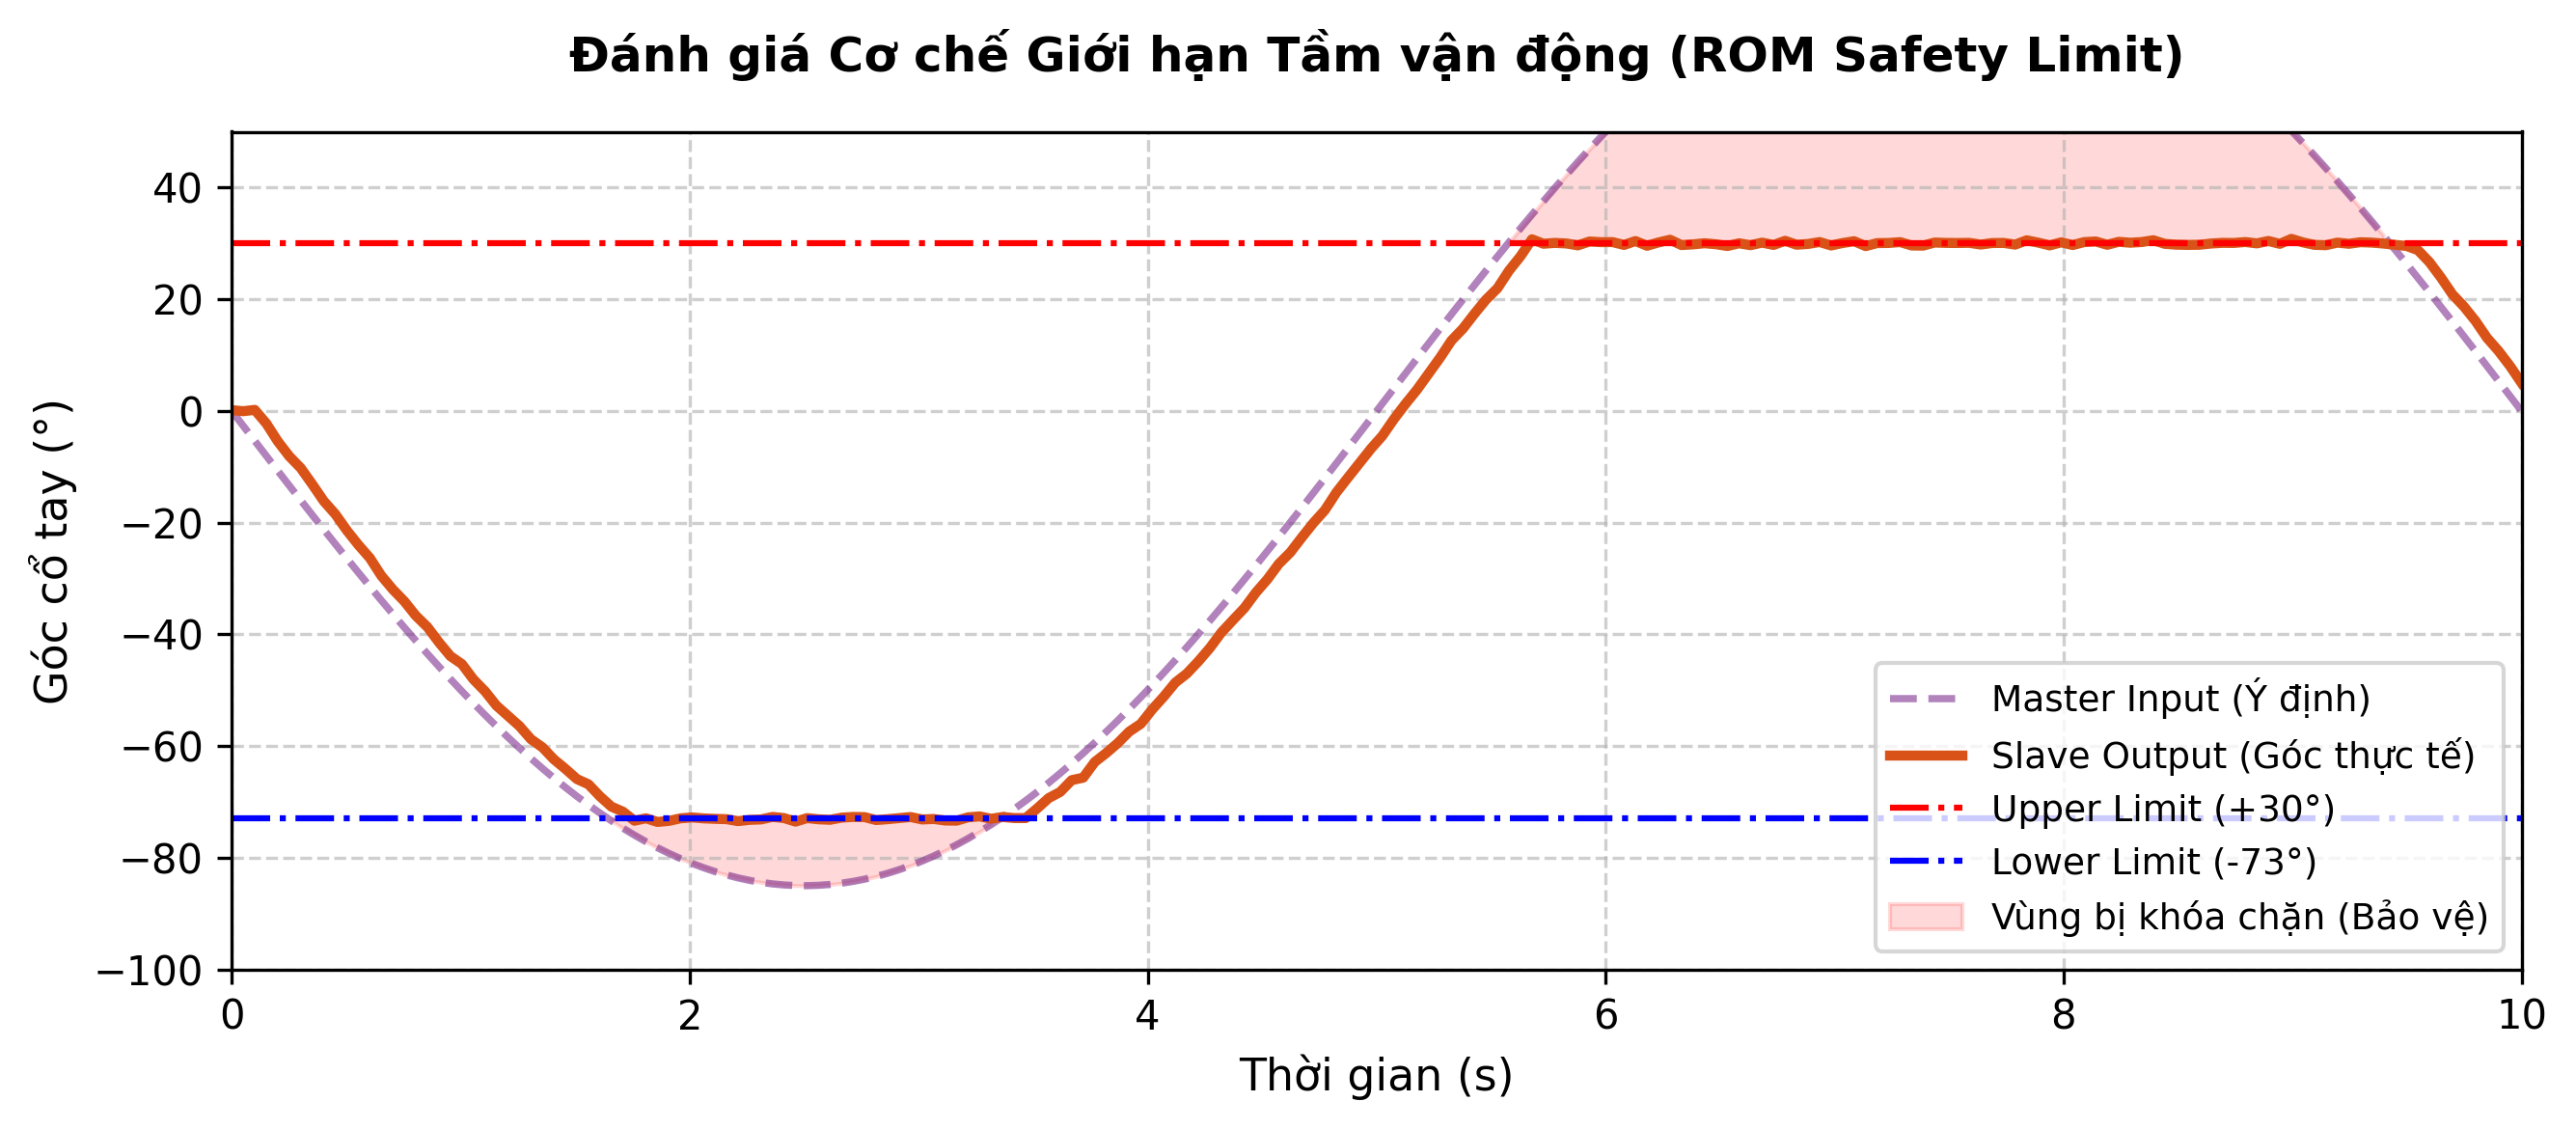
\includegraphics[width=\columnwidth]{bieudo2.png}
\caption{Plot illustrating the hardware safety bounding mechanism when the Master angle exceeds the ROM limit thresholds ($limitMin = -73^\circ, limitMax = 30^\circ$).}
\label{fig:safety_limit}
\end{figure}
% =======================================

In a scenario simulating a patient losing control of the trajectory, the hardware angles are statically limited via the two-point calibration algorithm (e.g., $limitMin = -73^\circ, limitMax = 30^\circ$). Measurement results in Fig. \ref{fig:safety_limit} confirm that even when the Master signal exceeds the threshold, the Slave coordinates remain precisely locked at the physical boundary, completely protecting the patient's wrist joint from potential injuries.

\section{Discussion}

The experimental results confirm the effectiveness of the "Zero-Setup" architecture in simplifying the interaction process between users and the rehabilitation device. Utilizing the Web Serial API not only reduces communication latency to an insignificant level (< 50ms) but also creates a uniform operating platform, allowing exercises to be deployed on any computer with a web browser without complex hardware configuration.

Regarding motion control, the position tracking plot (Fig. \ref{fig:dashboard}) shows that the combination of the PID controller and the S-Curve dead-zone compensation algorithm fundamentally resolved the static friction issues of the GA25 motor gearbox. This smooth motion trajectory is a prerequisite for ensuring patient comfort during passive range-of-motion exercises. Furthermore, the ROM safety bounding mechanism (Fig. \ref{fig:safety_limit}) serves as a reliable "physical protection layer," preventing any risk of injury due to software errors or loss of intentional control.

Regarding assistive force measurement, although the system has been designed with an integrated INA219 current sensor structure and mathematical models for torque estimation, this part is currently at the stage of theoretical realization and architectural design. Preliminary tests show that the system is ready in terms of data infrastructure to receive current feedback signals. However, to achieve precision in Impedance Control, the calibration of dynamic and static friction models based on actual current will require a more intensive experimental process. The future availability of force data layers will help the system transition from passive assistance to active assistance based on patient effort (Assist-as-needed).

\section{Conclusion and Future Work}

This research presented the successful design and implementation of a mechatronic wrist rehabilitation system focused on a "Zero-Setup" feature for home-based Telerehabilitation. By directly connecting hardware communication via a Master-Slave architecture to an HTML5 game interface through the Web Serial API, we have completely eliminated the requirement for complex software configuration—the largest technological barrier for elderly patients \cite{nikafrooz2017design}. The Kinematic Control system ensures smooth motion trajectories and maximum safety through mathematical hardware-level safety bounding mechanisms.

Although the hardware platform has integrated an INA219 current sensor along with cascaded filtering algorithms for torque estimation, this force monitoring mechanism is currently undergoing empirical calibration. In the next development phase, research will focus on quantitatively evaluating the accuracy of the force estimation mathematical model to formally activate the Impedance Control mode. This direction will expand the device's capabilities from mere Kinematic Tracking to providing active resistive force, helping to personalize physical therapy routines for various stages of neuromuscular recovery in stroke patients.

\begin{thebibliography}{1}

\bibitem{vo2024design}
C. Vo Duy, "Design and development of a wrist rehabilitation device with an interactive game," \textit{Results in Engineering}, vol. 22, p. 102336, 2024.

\bibitem{omarkulov2016preliminary}
N. Omarkulov, K. Telegenov, M. Zeinullin, I. Tursynbek, and A. Shintemirov, "Preliminary mechanical design of NU-Wrist: A 3-DOF self-aligning wrist rehabilitation robot," in \textit{2016 6th IEEE RAS/EMBS International Conference on Biomedical Robotics and Biomechatronics (BioRob)}, 2016, pp. 962-967.

\bibitem{tolks2024role}
D. Tolks, J. J. Schmidt, and S. Kuhn, "The Role of AI in Serious Games and Gamification for Health: Scoping Review," \textit{JMIR Serious Games}, vol. 12, p. e48258, 2024.

\bibitem{park2025effects}
J. M. Park et al., "Effects of Robot-Assisted Therapy for Upper Limb Rehabilitation After Stroke: An Umbrella Review of Systematic Reviews," \textit{Stroke}, vol. 56, no. 5, pp. 1239-1253, 2025.

\bibitem{nikafrooz2017design}
N. Nikafrooz, M. J. Mahjoob, and M. A. Tofigh, "Design, modeling, and fabrication of a 3-DOF wrist rehabilitation robot," in \textit{2017 IEEE International Conference on Rehabilitation Robotics (ICORR)}, 2017.

\bibitem{pezent2017design}
E. Pezent, C. G. Rose, A. D. Deshpande, and M. K. O'Malley, "Design and characterization of the OpenWrist: A robotic wrist exoskeleton for coordinated hand-wrist rehabilitation," in \textit{2017 International Conference on Rehabilitation Robotics (ICORR)}, 2017, pp. 720-725.

\end{thebibliography}

\end{document}
